% Options for packages loaded elsewhere
\PassOptionsToPackage{unicode}{hyperref}
\PassOptionsToPackage{hyphens}{url}
\PassOptionsToPackage{dvipsnames,svgnames,x11names}{xcolor}
%
\documentclass[
  letterpaper,
  DIV=11,
  numbers=noendperiod]{scrartcl}

\usepackage{amsmath,amssymb}
\usepackage{iftex}
\ifPDFTeX
  \usepackage[T1]{fontenc}
  \usepackage[utf8]{inputenc}
  \usepackage{textcomp} % provide euro and other symbols
\else % if luatex or xetex
  \usepackage{unicode-math}
  \defaultfontfeatures{Scale=MatchLowercase}
  \defaultfontfeatures[\rmfamily]{Ligatures=TeX,Scale=1}
\fi
\usepackage{lmodern}
\ifPDFTeX\else  
    % xetex/luatex font selection
\fi
% Use upquote if available, for straight quotes in verbatim environments
\IfFileExists{upquote.sty}{\usepackage{upquote}}{}
\IfFileExists{microtype.sty}{% use microtype if available
  \usepackage[]{microtype}
  \UseMicrotypeSet[protrusion]{basicmath} % disable protrusion for tt fonts
}{}
\makeatletter
\@ifundefined{KOMAClassName}{% if non-KOMA class
  \IfFileExists{parskip.sty}{%
    \usepackage{parskip}
  }{% else
    \setlength{\parindent}{0pt}
    \setlength{\parskip}{6pt plus 2pt minus 1pt}}
}{% if KOMA class
  \KOMAoptions{parskip=half}}
\makeatother
\usepackage{xcolor}
\setlength{\emergencystretch}{3em} % prevent overfull lines
\setcounter{secnumdepth}{5}
% Make \paragraph and \subparagraph free-standing
\makeatletter
\ifx\paragraph\undefined\else
  \let\oldparagraph\paragraph
  \renewcommand{\paragraph}{
    \@ifstar
      \xxxParagraphStar
      \xxxParagraphNoStar
  }
  \newcommand{\xxxParagraphStar}[1]{\oldparagraph*{#1}\mbox{}}
  \newcommand{\xxxParagraphNoStar}[1]{\oldparagraph{#1}\mbox{}}
\fi
\ifx\subparagraph\undefined\else
  \let\oldsubparagraph\subparagraph
  \renewcommand{\subparagraph}{
    \@ifstar
      \xxxSubParagraphStar
      \xxxSubParagraphNoStar
  }
  \newcommand{\xxxSubParagraphStar}[1]{\oldsubparagraph*{#1}\mbox{}}
  \newcommand{\xxxSubParagraphNoStar}[1]{\oldsubparagraph{#1}\mbox{}}
\fi
\makeatother

\usepackage{color}
\usepackage{fancyvrb}
\newcommand{\VerbBar}{|}
\newcommand{\VERB}{\Verb[commandchars=\\\{\}]}
\DefineVerbatimEnvironment{Highlighting}{Verbatim}{commandchars=\\\{\}}
% Add ',fontsize=\small' for more characters per line
\usepackage{framed}
\definecolor{shadecolor}{RGB}{241,243,245}
\newenvironment{Shaded}{\begin{snugshade}}{\end{snugshade}}
\newcommand{\AlertTok}[1]{\textcolor[rgb]{0.68,0.00,0.00}{#1}}
\newcommand{\AnnotationTok}[1]{\textcolor[rgb]{0.37,0.37,0.37}{#1}}
\newcommand{\AttributeTok}[1]{\textcolor[rgb]{0.40,0.45,0.13}{#1}}
\newcommand{\BaseNTok}[1]{\textcolor[rgb]{0.68,0.00,0.00}{#1}}
\newcommand{\BuiltInTok}[1]{\textcolor[rgb]{0.00,0.23,0.31}{#1}}
\newcommand{\CharTok}[1]{\textcolor[rgb]{0.13,0.47,0.30}{#1}}
\newcommand{\CommentTok}[1]{\textcolor[rgb]{0.37,0.37,0.37}{#1}}
\newcommand{\CommentVarTok}[1]{\textcolor[rgb]{0.37,0.37,0.37}{\textit{#1}}}
\newcommand{\ConstantTok}[1]{\textcolor[rgb]{0.56,0.35,0.01}{#1}}
\newcommand{\ControlFlowTok}[1]{\textcolor[rgb]{0.00,0.23,0.31}{\textbf{#1}}}
\newcommand{\DataTypeTok}[1]{\textcolor[rgb]{0.68,0.00,0.00}{#1}}
\newcommand{\DecValTok}[1]{\textcolor[rgb]{0.68,0.00,0.00}{#1}}
\newcommand{\DocumentationTok}[1]{\textcolor[rgb]{0.37,0.37,0.37}{\textit{#1}}}
\newcommand{\ErrorTok}[1]{\textcolor[rgb]{0.68,0.00,0.00}{#1}}
\newcommand{\ExtensionTok}[1]{\textcolor[rgb]{0.00,0.23,0.31}{#1}}
\newcommand{\FloatTok}[1]{\textcolor[rgb]{0.68,0.00,0.00}{#1}}
\newcommand{\FunctionTok}[1]{\textcolor[rgb]{0.28,0.35,0.67}{#1}}
\newcommand{\ImportTok}[1]{\textcolor[rgb]{0.00,0.46,0.62}{#1}}
\newcommand{\InformationTok}[1]{\textcolor[rgb]{0.37,0.37,0.37}{#1}}
\newcommand{\KeywordTok}[1]{\textcolor[rgb]{0.00,0.23,0.31}{\textbf{#1}}}
\newcommand{\NormalTok}[1]{\textcolor[rgb]{0.00,0.23,0.31}{#1}}
\newcommand{\OperatorTok}[1]{\textcolor[rgb]{0.37,0.37,0.37}{#1}}
\newcommand{\OtherTok}[1]{\textcolor[rgb]{0.00,0.23,0.31}{#1}}
\newcommand{\PreprocessorTok}[1]{\textcolor[rgb]{0.68,0.00,0.00}{#1}}
\newcommand{\RegionMarkerTok}[1]{\textcolor[rgb]{0.00,0.23,0.31}{#1}}
\newcommand{\SpecialCharTok}[1]{\textcolor[rgb]{0.37,0.37,0.37}{#1}}
\newcommand{\SpecialStringTok}[1]{\textcolor[rgb]{0.13,0.47,0.30}{#1}}
\newcommand{\StringTok}[1]{\textcolor[rgb]{0.13,0.47,0.30}{#1}}
\newcommand{\VariableTok}[1]{\textcolor[rgb]{0.07,0.07,0.07}{#1}}
\newcommand{\VerbatimStringTok}[1]{\textcolor[rgb]{0.13,0.47,0.30}{#1}}
\newcommand{\WarningTok}[1]{\textcolor[rgb]{0.37,0.37,0.37}{\textit{#1}}}

\providecommand{\tightlist}{%
  \setlength{\itemsep}{0pt}\setlength{\parskip}{0pt}}\usepackage{longtable,booktabs,array}
\usepackage{calc} % for calculating minipage widths
% Correct order of tables after \paragraph or \subparagraph
\usepackage{etoolbox}
\makeatletter
\patchcmd\longtable{\par}{\if@noskipsec\mbox{}\fi\par}{}{}
\makeatother
% Allow footnotes in longtable head/foot
\IfFileExists{footnotehyper.sty}{\usepackage{footnotehyper}}{\usepackage{footnote}}
\makesavenoteenv{longtable}
\usepackage{graphicx}
\makeatletter
\def\maxwidth{\ifdim\Gin@nat@width>\linewidth\linewidth\else\Gin@nat@width\fi}
\def\maxheight{\ifdim\Gin@nat@height>\textheight\textheight\else\Gin@nat@height\fi}
\makeatother
% Scale images if necessary, so that they will not overflow the page
% margins by default, and it is still possible to overwrite the defaults
% using explicit options in \includegraphics[width, height, ...]{}
\setkeys{Gin}{width=\maxwidth,height=\maxheight,keepaspectratio}
% Set default figure placement to htbp
\makeatletter
\def\fps@figure{htbp}
\makeatother

\usepackage{booktabs}
\usepackage{longtable}
\usepackage{array}
\usepackage{multirow}
\usepackage{wrapfig}
\usepackage{float}
\usepackage{colortbl}
\usepackage{pdflscape}
\usepackage{tabu}
\usepackage{threeparttable}
\usepackage{threeparttablex}
\usepackage[normalem]{ulem}
\usepackage{makecell}
\usepackage{xcolor}
\KOMAoption{captions}{tableheading}
\usepackage{amsmath}
\usepackage{amssymb}
\usepackage{pgfplots}
\usepackage[top=0.5in, bottom=1in, left=1in, right=1in]{geometry}
\makeatletter
\@ifpackageloaded{caption}{}{\usepackage{caption}}
\AtBeginDocument{%
\ifdefined\contentsname
  \renewcommand*\contentsname{Table of contents}
\else
  \newcommand\contentsname{Table of contents}
\fi
\ifdefined\listfigurename
  \renewcommand*\listfigurename{List of Figures}
\else
  \newcommand\listfigurename{List of Figures}
\fi
\ifdefined\listtablename
  \renewcommand*\listtablename{List of Tables}
\else
  \newcommand\listtablename{List of Tables}
\fi
\ifdefined\figurename
  \renewcommand*\figurename{Figure}
\else
  \newcommand\figurename{Figure}
\fi
\ifdefined\tablename
  \renewcommand*\tablename{Table}
\else
  \newcommand\tablename{Table}
\fi
}
\@ifpackageloaded{float}{}{\usepackage{float}}
\floatstyle{ruled}
\@ifundefined{c@chapter}{\newfloat{codelisting}{h}{lop}}{\newfloat{codelisting}{h}{lop}[chapter]}
\floatname{codelisting}{Listing}
\newcommand*\listoflistings{\listof{codelisting}{List of Listings}}
\makeatother
\makeatletter
\makeatother
\makeatletter
\@ifpackageloaded{caption}{}{\usepackage{caption}}
\@ifpackageloaded{subcaption}{}{\usepackage{subcaption}}
\makeatother

\ifLuaTeX
  \usepackage{selnolig}  % disable illegal ligatures
\fi
\usepackage{bookmark}

\IfFileExists{xurl.sty}{\usepackage{xurl}}{} % add URL line breaks if available
\urlstyle{same} % disable monospaced font for URLs
\hypersetup{
  pdftitle={Impact of Caffeinated and Caffeine-Free Beverages on the Problem Solving Skills of A Virtual Population},
  pdfauthor={Bhagatinder Longia; Musab Muhammad; Muntasir Munem; Shea Munson; Chloe Syriac},
  colorlinks=true,
  linkcolor={blue},
  filecolor={Maroon},
  citecolor={Blue},
  urlcolor={Blue},
  pdfcreator={LaTeX via pandoc}}


\title{Impact of Caffeinated and Caffeine-Free Beverages on the Problem
Solving Skills of A Virtual Population\thanks{Data available at
\url{https://github.com/shea-m/Beverage-Impact-on-Problem-Solving-STA305H5S2025}}}
\usepackage{etoolbox}
\makeatletter
\providecommand{\subtitle}[1]{% add subtitle to \maketitle
  \apptocmd{\@title}{\par {\large #1 \par}}{}{}
}
\makeatother
\subtitle{Study for STA305 at University of Toronto Mississauga}
\author{Bhagatinder Longia \and Musab Muhammad \and Muntasir
Munem \and Shea Munson \and Chloe Syriac}
\date{March 19, 2025}

\begin{document}
\maketitle
\begin{abstract}
Caffeine is the most popular psychoactive substance in the world,
particularly due to its widely known stimulating effects. As a
stimulant, caffeine has mostly commonly been used to increase mental
alertness, which is why the goal of our study is to determine if there
is an association between caffeine use and problem solving skills. We
collected data using a virtual population on The Islands. After
collecting a sample of 150 virtual participants and splitting them into
three age groups, a caffeinated or caffeine-free drink, with water as a
control, were administered to each participant. Using a balanced
Kruskal-Wallis test, we found that {[}summary of key findings{]}.
{[}brief overview of result implications, improvments needed{]}.
\end{abstract}

\renewcommand*\contentsname{Table of contents}
{
\hypersetup{linkcolor=}
\setcounter{tocdepth}{3}
\tableofcontents
}

\newpage

\section{Introduction}\label{introduction}

As the world's most popular psychoactive substance, caffeine's widely
known effects have been studied extensively. Despite certain drawbacks
like digestion and anxiety issues in some people, due to being a
stimulant, it has most commonly been used to temporarily increase mental
alertness which improves things like memory and lessens fatigue, thus
providing an energy boost.

In this study, we are analyzing whether there is an association between
caffeine use and problem solving skills by giving coffee, energy drinks,
and caffeine-free versions of both to participants from the
\href{https://islands.smp.uq.edu.au/}{The Islands}, a virtual population
developed by the University of Queensland for learning and teaching in
statistics. Our sample was split into three age groups: 18-35, 36-54,
and 55+. Considering the effects of caffeine, participants assigned a
caffeinated drink would be expected to achieve a higher score that those
that are not.

We aim to study the following research questions:

\begin{itemize}
\item
  Research Question 1 (RQ1): Does beverage type have an impact on
  problem solving score?

  \begin{itemize}
  \item
    \(H_{0}\): no association between beverage type and problem solving
    score.
  \item
    \(H_{a}\): association between beverage type and problem solving
    score exists.
  \end{itemize}
\item
  Research Question 2 (RQ2): Do caffeinated coffee and energy drinks
  have a higher impact on problem solving scores compared to their
  caffeine-free counterparts?

  \begin{itemize}
  \item
    \(H_{0}\): no association between caffeinated drinks and higher
    score
  \item
    \(H_{a}\): association between caffeinated drinks and higher score
    exists.
  \end{itemize}
\end{itemize}

This paper consist of our methodology, analysis, results, limitations,
and a conclusion for our study.

\section{Methodology}\label{methodology}

\subsection{Design and Setup}\label{design-and-setup}

In February 2025, we conducted an experiment to determine if different
caffeinated and caffeine-free drinks effect the problem solving skills
of virtual participants on The Islands. Our experiment utilized a
balanced one-way randomized complete block (RCB) design. Participants
were blocked out into one of three age groups, where they were given one
of five drinks (the treatment) and had their score on a 20 minute
problem solving test (the response) recorded.

Each of the three age group blocks contained an equal number of
participants for each treatment, per our RCB design. While we did not
have any major factors that we could easily control for, to help account
for nuisance factors treatments were randomly assigned among
participants using an R script (See Listing~\ref{lst-rand} in Appendix).

The experiment included a total of 150 participants \((n = 150)\), with
50 in each of the following age blocks: 18-35, 36-54, and 55+. Each
participant was given one of five 250 millilitre drinks \((a = 5)\):
Water (Control), Energy Drink, Energy Drink Decaffeinated, Coffee, or
Coffee Decaffeinated. Each treatment factor contained 30 participants
\((n_j = 30)\), split evenly among the three age blocks thus giving a
balanced design. This also provided for enough repetitions to further
account for nuisance factors that might not have been dealt with through
the blocking or randomization. Since each participant was exposed to
only one treatment and randomly assigned to a treatment group, this
experiment utilized a between-subjects design.

\subsection{Data Collection}\label{data-collection}

Each participant was given their randomly assigned drink and then
administered a 20 minute problem solving test. The test was scored from
0 to 100 and after completion, each participants score was recorded.
Once all data collection was completed, it was cleaned, stripping any
personally identifying information and assigning factor levels and names
more easily utilizable and readable within R.

\section{Analysis}\label{analysis}

\subsection{Summary Statistics and Checking
Assumptions}\label{summary-statistics-and-checking-assumptions}

We began by gathering summary statistics of our data, presented in
Table~\ref{tbl-table1}. The high mean and median indicate that
participants generally scored well on the problem solving test. A low
standard deviation indicates tight clustering around the mean and a low
IQR indicates tight clustering around the median. The minimum of 67 lies
well outside of 1.5 \(\times\) IQR, indicating a presence of outliers on
the low side, with further inspection necessary to determine the amount.
The maximum of 100 along with the data being skewed to the high means
that there are no outliers present on the high end.

\begin{longtable}[]{@{}lcccccc@{}}

\caption{\label{tbl-table1}Summary of Problem Solving Test Scores}

\tabularnewline

\toprule\noalign{}
& Min & Max & Mean & Median & SD & IQR \\
\midrule\noalign{}
\endhead
\bottomrule\noalign{}
\endlastfoot
Value & 67 & 100 & 93.4867 & 96 & 6.9618 & 6.75 \\

\end{longtable}

More preliminary information is obtained plotting the treatments in
relation to scores in Figure~\ref{fig-boxplot1}.

\begin{figure}[H]

\centering{

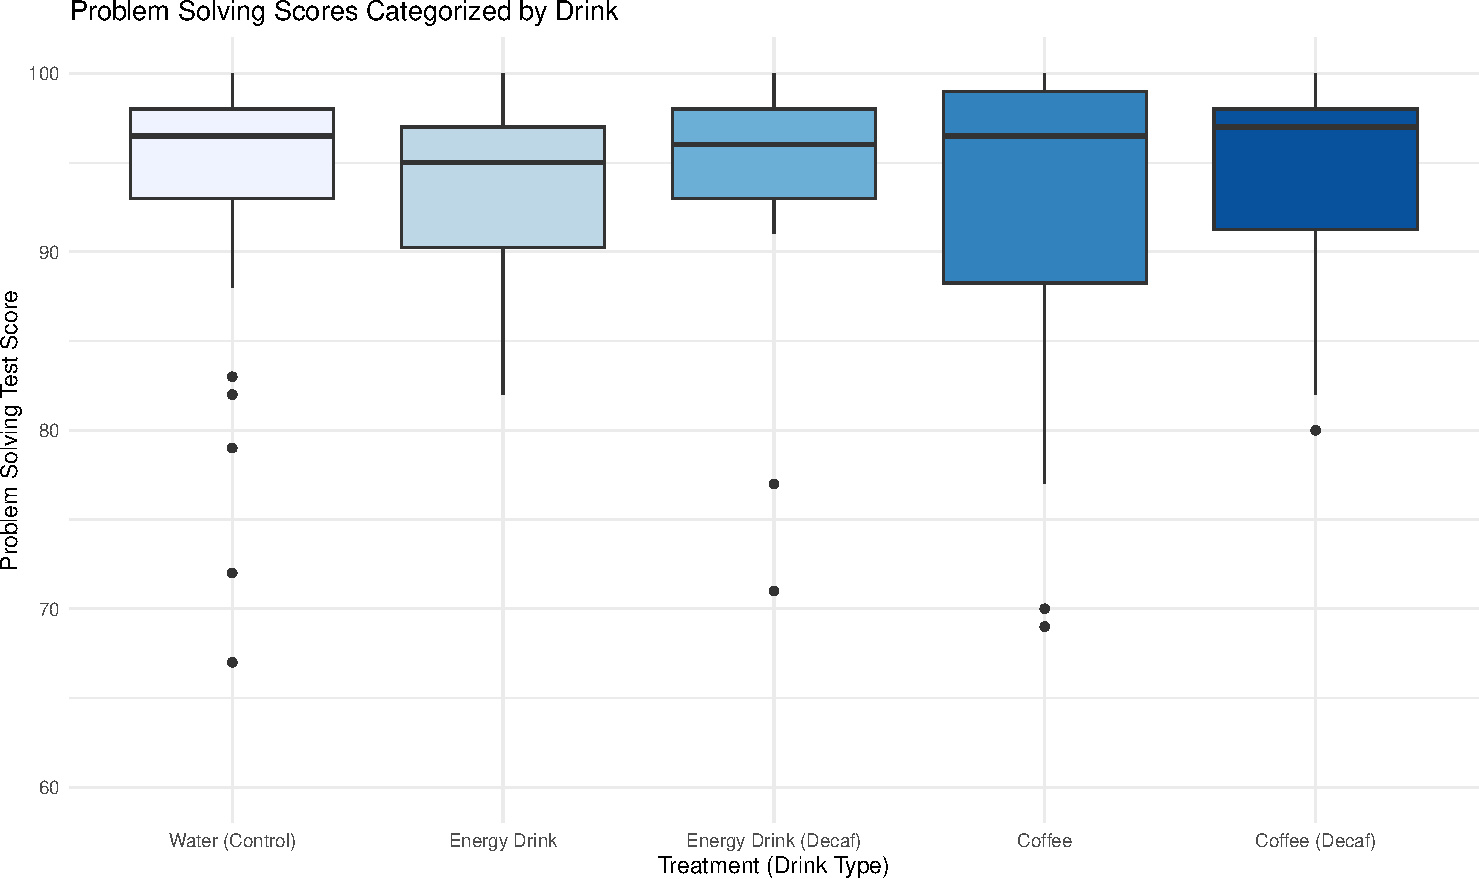
\includegraphics{the_residuals_technical_report_files/figure-pdf/fig-boxplot1-1.pdf}

}

\caption{\label{fig-boxplot1}Boxplot of Scores by Treatment}

\end{figure}%

From the boxplot, we can make an initial inference that the means are
likely similar among groups, however the variances are different. To
confirm this, further analysis will be utilized, but prior to that we
must check assumptions to determine if a one-way ANOVA can be utilized,
or if we must proceed with a Kruskal-Wallis non-parametric test. The
three assumptions that must be checked are independence, normally
distributed, and homogeneous variance.

\begin{enumerate}
\def\labelenumi{\arabic{enumi}.}
\tightlist
\item
  Independence: This assumption is satisfied by design. All data points
  are collected from unique individuals whose results do not depend on
  the others.
\item
  Normality: Violated, as seen in Figure~\ref{fig-checks}
\item
  Homogeneity of Variance: Violated, as seen in Figure~\ref{fig-checks}
\end{enumerate}

\begin{figure}[H]

\centering{

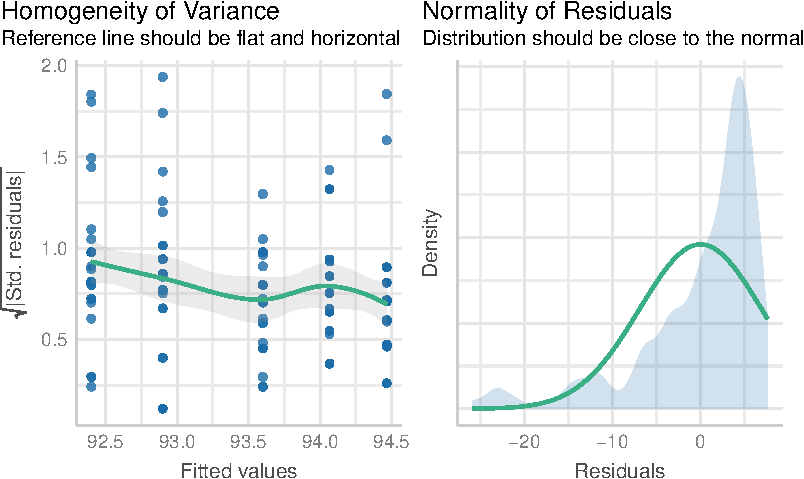
\includegraphics{the_residuals_technical_report_files/figure-pdf/fig-checks-1.pdf}

}

\caption{\label{fig-checks}Checking One-Way ANOVA Assumptions (Visual)}

\end{figure}%

\begin{table}

\caption{\label{tbl-checks}}

\centering{

\begin{figure}
\centering
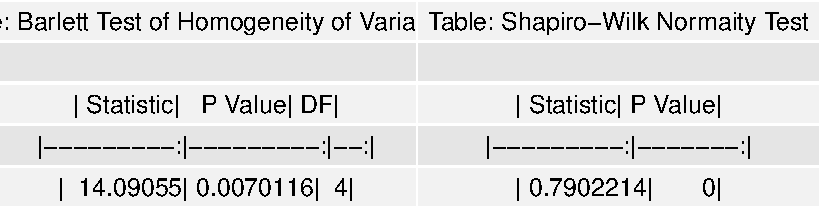
\includegraphics{the_residuals_technical_report_files/figure-pdf/tbl-checks-1.pdf}
\caption{Checking One-Way ANOVA Assumptions (P Values)}
\end{figure}

}

\end{table}%

\subsection{Statistical Tests}\label{statistical-tests}

As the assumption of normality and homogeneity of variance have been
violated, we are unable to use a one-way ANOVA test. Instead, we opt to
use Kruskal-Wallis non-parametric H-test utilizing the treatment type
(beverage given) as our factor. The results of the Kruskal-Wallis H-test
are displayed below in Table~\ref{tbl-kwtest}.

\begin{longtable}[]{@{}rrr@{}}

\caption{\label{tbl-kwtest}Kruskal-Wallis H-Test}

\tabularnewline

\toprule\noalign{}
H-Statistic & P Value & DF \\
\midrule\noalign{}
\endhead
\bottomrule\noalign{}
\endlastfoot
1.811637 & 0.7703527 & 4 \\

\end{longtable}

\section{Results}\label{results}

From Table~\ref{tbl-kwtest} we find a p-value for the Kruskal-Wallis
H-test is 0.7735. This p-value is significantly greater than our
significance level of \(\alpha = 0.05\). As a result, there is not any
statistically significant level evidence to suggest the mean problem
solving score is different among treatment groups. This result is to be
expected as it confirms the initial results inferred from
Figure~\ref{fig-boxplot1}.

Since there we're no significant results, no further followup was
necessary for RQ2. If there were statistically significant differences
in caffeinated vs non-caffeinated beverages, we would have also seen
statistically significant evidence that the means among drinks was not
equal.

\section{Limitations}\label{limitations}

This study had a number of limitations. One thing that should have done
differently was waiting after giving each participant their beverage
before administering the problem solving test. We administered the test
immediately after giving participants their treatment, which could have
impacted results. Waiting would have allowed for more absorption of
caffeine and therefore a better look into its impact.

Additionally, despite the depth provided by The Islands for conducting
an experiment, using a virtual population is a major limitation in
assessing the impact of caffeine on the problem solving skills of real
people. This is because it does not take all of the countless real life
factors that impact caffeine into account. Further, we do not know
exactly the implementation of the problem solving quiz or the drinks,
resulting in a significant level of unknown. As a result, our experiment
may not be incredibly relevant to the real world.

The final major limitation we had was the model used. We would have like
to utilize a two-way ANOVA model, with drink and age as factors, as
Figure~\ref{fig-dblboxplot} indicates there might be some difference
among different drinks between age groups.

\begin{figure}[H]

\centering{

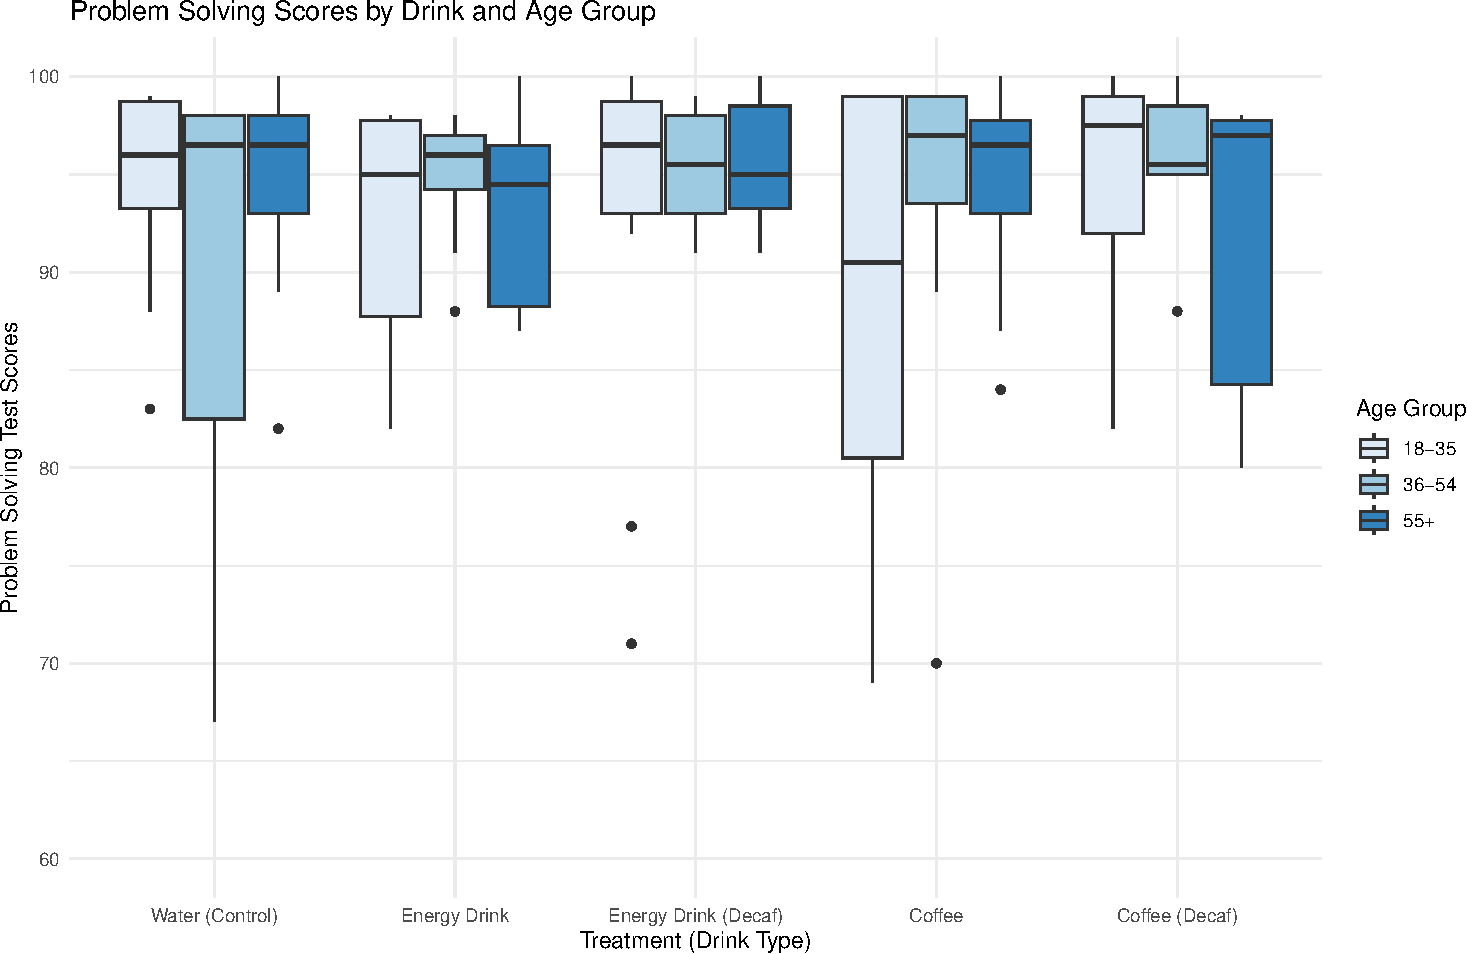
\includegraphics{the_residuals_technical_report_files/figure-pdf/fig-dblboxplot-1.pdf}

}

\caption{\label{fig-dblboxplot}Box Plot Showing Problem Solving Scores
by Drink and Age Group}

\end{figure}%

Unfortunately, similar to one-way, our assumptions for both normality
and homogeneity of variance were violated, shown in
Figure~\ref{fig-twowaychecks}. Due to the challenge of implementing a
non-parametric two-way ANOVA test and because of time constraints, we
were unfortunately unable to implement this model and had to instead
utilize the one-way Kruskal-Wallis model.

\begin{figure}[H]

\centering{

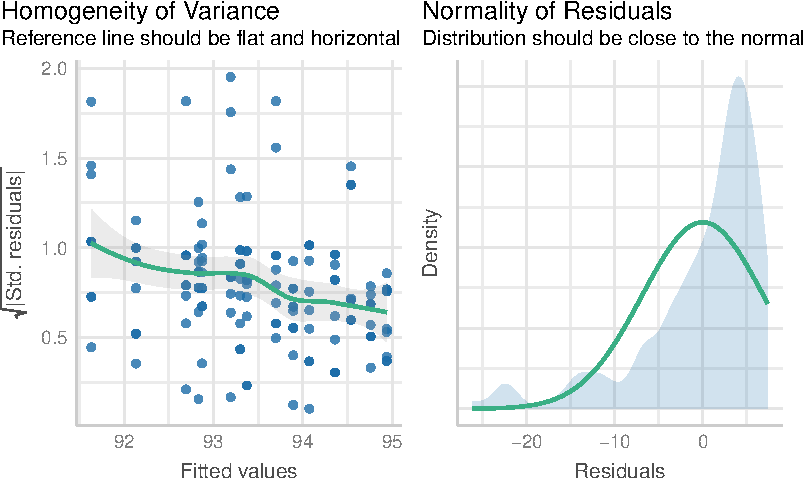
\includegraphics{the_residuals_technical_report_files/figure-pdf/fig-twowaychecks-1.pdf}

}

\caption{\label{fig-twowaychecks}}

\end{figure}%

\section{Conclusion}\label{conclusion}

This study aimed to examine the potential association between caffeine
consumption through various beverages and problem-solving performance
scores among virtual participants in The Islands. Analysis from a sample
of 150 participants showed {[}include key findings.{]}

\section{Appendix}\label{appendix}

\begin{codelisting}

\caption{\label{lst-rand}Randomization Script for Assigning Treatments}

\centering{

\begin{Shaded}
\begin{Highlighting}[]
\FunctionTok{library}\NormalTok{(clipr)}
\NormalTok{groups }\OtherTok{\textless{}{-}} \FunctionTok{c}\NormalTok{(}\StringTok{"Water"}\NormalTok{, }\StringTok{"Coffee"}\NormalTok{, }\StringTok{"Coffee (Decaf)"}\NormalTok{, }\StringTok{"Energy Drink"}\NormalTok{, }
          \StringTok{"Energy Drink (Decaf)"}\NormalTok{)}
\NormalTok{labels }\OtherTok{\textless{}{-}} \FunctionTok{rep}\NormalTok{(groups, }\DecValTok{10}\NormalTok{)}
\NormalTok{shuffled }\OtherTok{\textless{}{-}} \FunctionTok{sample}\NormalTok{(labels)}
\FunctionTok{write\_clip}\NormalTok{(shuffled, }\AttributeTok{type =} \StringTok{"text"}\NormalTok{)}
\end{Highlighting}
\end{Shaded}

}

\end{codelisting}%

\begin{Shaded}
\begin{Highlighting}[]
\CommentTok{\# Ensure necessary packages are installed and loaded}
\NormalTok{packages }\OtherTok{\textless{}{-}} \FunctionTok{c}\NormalTok{(}\StringTok{"tidyverse"}\NormalTok{, }\StringTok{"patchwork"}\NormalTok{, }\StringTok{"performance"}\NormalTok{, }\StringTok{"knitr"}\NormalTok{, }\StringTok{"see"}\NormalTok{, }
              \StringTok{"kableExtra"}\NormalTok{, }\StringTok{"broom"}\NormalTok{)}
\ControlFlowTok{for}\NormalTok{(pkg }\ControlFlowTok{in}\NormalTok{ packages) \{}
  \ControlFlowTok{if}\NormalTok{ (}\SpecialCharTok{!}\FunctionTok{requireNamespace}\NormalTok{(pkg, }\AttributeTok{quietly =} \ConstantTok{TRUE}\NormalTok{)) \{}
    \FunctionTok{install.packages}\NormalTok{(pkg)}
\NormalTok{  \}}
\NormalTok{\}}
\FunctionTok{library}\NormalTok{(tidyverse)}
\FunctionTok{library}\NormalTok{(patchwork)}
\FunctionTok{library}\NormalTok{(performance)}
\FunctionTok{library}\NormalTok{(knitr)}
\FunctionTok{library}\NormalTok{(see)}
\FunctionTok{library}\NormalTok{(kableExtra)}
\FunctionTok{library}\NormalTok{(broom)}

\CommentTok{\# Load the Data}
\NormalTok{data }\OtherTok{\textless{}{-}} \FunctionTok{read.csv}\NormalTok{(}\StringTok{"cleaned\_data.csv"}\NormalTok{, }\AttributeTok{header =} \ConstantTok{TRUE}\NormalTok{)}

\CommentTok{\# Put factor levels in desired order}
\NormalTok{data}\SpecialCharTok{$}\NormalTok{age\_group }\OtherTok{\textless{}{-}} \FunctionTok{factor}\NormalTok{(data}\SpecialCharTok{$}\NormalTok{age\_group, }
                         \AttributeTok{levels =} \FunctionTok{c}\NormalTok{(}\StringTok{"Y"}\NormalTok{, }\StringTok{"M"}\NormalTok{, }\StringTok{"O"}\NormalTok{), }
                         \AttributeTok{labels =} \FunctionTok{c}\NormalTok{(}\StringTok{"18{-}35"}\NormalTok{, }\StringTok{"36{-}54"}\NormalTok{, }\StringTok{"55+"}\NormalTok{))}
\NormalTok{data}\SpecialCharTok{$}\NormalTok{treatment }\OtherTok{\textless{}{-}} \FunctionTok{factor}\NormalTok{(data}\SpecialCharTok{$}\NormalTok{treatment, }
                         \AttributeTok{levels =} \FunctionTok{c}\NormalTok{(}\StringTok{"W"}\NormalTok{, }\StringTok{"E"}\NormalTok{, }\StringTok{"ED"}\NormalTok{, }\StringTok{"C"}\NormalTok{, }\StringTok{"CD"}\NormalTok{), }
                         \AttributeTok{labels =} \FunctionTok{c}\NormalTok{(}\StringTok{"Water (Control)"}\NormalTok{, }\StringTok{"Energy Drink"}\NormalTok{, }
                                    \StringTok{"Energy Drink (Decaf)"}\NormalTok{, }\StringTok{"Coffee"}\NormalTok{, }
                                    \StringTok{"Coffee (Decaf)"}\NormalTok{))}
\FunctionTok{attach}\NormalTok{(data)}

\CommentTok{\# Generate table for score summary data}
\NormalTok{sum\_data }\OtherTok{\textless{}{-}} \FunctionTok{data.frame}\NormalTok{(}\AttributeTok{Value =} \FunctionTok{c}\NormalTok{(}\FunctionTok{min}\NormalTok{(score), }\FunctionTok{max}\NormalTok{(score), }\FunctionTok{round}\NormalTok{(}\FunctionTok{mean}\NormalTok{(score), }\DecValTok{4}\NormalTok{), }
                                 \FunctionTok{median}\NormalTok{(score), }\FunctionTok{round}\NormalTok{(}\FunctionTok{sd}\NormalTok{(score), }\DecValTok{4}\NormalTok{), }\FunctionTok{IQR}\NormalTok{(score)))}
\NormalTok{labs }\OtherTok{\textless{}{-}} \FunctionTok{c}\NormalTok{(}\StringTok{"Min"}\NormalTok{, }\StringTok{"Max"}\NormalTok{, }\StringTok{"Mean"}\NormalTok{, }\StringTok{"Median"}\NormalTok{, }\StringTok{"SD"}\NormalTok{, }\StringTok{"IQR"}\NormalTok{)}
\FunctionTok{kable}\NormalTok{(}\FunctionTok{t}\NormalTok{(sum\_data), }\AttributeTok{col.names =}\NormalTok{ labs, }\AttributeTok{align =} \StringTok{"c"}\NormalTok{)}

\CommentTok{\# Generate boxplot for scores explained by drink}
\FunctionTok{ggplot}\NormalTok{(data, }\FunctionTok{aes}\NormalTok{(}\AttributeTok{x =}\NormalTok{ treatment, }\AttributeTok{y =}\NormalTok{ score, }\AttributeTok{fill =}\NormalTok{ treatment)) }\SpecialCharTok{+}
  \FunctionTok{geom\_boxplot}\NormalTok{() }\SpecialCharTok{+}
  \FunctionTok{scale\_y\_continuous}\NormalTok{(}\AttributeTok{limits =} \FunctionTok{c}\NormalTok{(}\DecValTok{60}\NormalTok{, }\DecValTok{100}\NormalTok{)) }\SpecialCharTok{+}
  \FunctionTok{scale\_fill\_brewer}\NormalTok{(}\AttributeTok{palette =} \StringTok{"Set1"}\NormalTok{) }\SpecialCharTok{+}
  \FunctionTok{labs}\NormalTok{(}\AttributeTok{title =} \StringTok{"Problem Solving Scores Categorized by Drink"}\NormalTok{,}
  \AttributeTok{x =} \StringTok{"Treatment (Drink Type)"}\NormalTok{, }\AttributeTok{y =} \StringTok{"Problem Solving Test Score"}\NormalTok{) }\SpecialCharTok{+}
  \FunctionTok{theme}\NormalTok{(}\AttributeTok{legend.position =} \StringTok{"none"}\NormalTok{)}

\CommentTok{\# Check assumptions for one{-}way model}
\NormalTok{one\_factor\_model }\OtherTok{\textless{}{-}} \FunctionTok{aov}\NormalTok{(score }\SpecialCharTok{\textasciitilde{}}\NormalTok{ treatment, }\AttributeTok{data =}\NormalTok{ data)}
\FunctionTok{check\_model}\NormalTok{(one\_factor\_model, }\AttributeTok{check =} \FunctionTok{c}\NormalTok{(}\StringTok{"normality"}\NormalTok{, }\StringTok{"homogeneity"}\NormalTok{))  }

\CommentTok{\# Perform non{-}parametric K{-}W test}
\NormalTok{non\_par }\OtherTok{\textless{}{-}} \FunctionTok{kruskal.test}\NormalTok{(score}\SpecialCharTok{\textasciitilde{}}\NormalTok{treatment, data)}
\NormalTok{formatted }\OtherTok{\textless{}{-}} \FunctionTok{as.data.frame}\NormalTok{(}\FunctionTok{tidy}\NormalTok{(non\_par))}
\NormalTok{formatted}\SpecialCharTok{$}\NormalTok{method }\OtherTok{\textless{}{-}} \ConstantTok{NULL}
\NormalTok{col\_names }\OtherTok{\textless{}{-}} \FunctionTok{c}\NormalTok{(}\StringTok{"H{-}Statistic"}\NormalTok{, }\StringTok{"P Value"}\NormalTok{, }\StringTok{"DF"}\NormalTok{)}
\FunctionTok{kable}\NormalTok{(formatted, }\AttributeTok{col.names =}\NormalTok{ col\_names, }
      \AttributeTok{caption =} \StringTok{"Kruskal{-}Wallis H{-}Test"}\NormalTok{)}

\CommentTok{\# Generate boxplot for scores explained by drink and age}
\NormalTok{age }\OtherTok{\textless{}{-}} \FunctionTok{c}\NormalTok{(}\StringTok{"18{-}35"}\NormalTok{, }\StringTok{"36{-}54"}\NormalTok{, }\StringTok{"55+"}\NormalTok{)}
\FunctionTok{ggplot}\NormalTok{(data, }\FunctionTok{aes}\NormalTok{(}\AttributeTok{x =}\NormalTok{ treatment, }\AttributeTok{y =}\NormalTok{ score, }\AttributeTok{fill =}\NormalTok{ age\_group)) }\SpecialCharTok{+}
  \FunctionTok{geom\_boxplot}\NormalTok{(}\AttributeTok{position =} \FunctionTok{position\_dodge}\NormalTok{(}\AttributeTok{width =} \FloatTok{0.8}\NormalTok{)) }\SpecialCharTok{+} 
  \FunctionTok{scale\_y\_continuous}\NormalTok{(}\AttributeTok{limits =} \FunctionTok{c}\NormalTok{(}\DecValTok{60}\NormalTok{, }\DecValTok{100}\NormalTok{)) }\SpecialCharTok{+} 
  \FunctionTok{labs}\NormalTok{(}\AttributeTok{title =} \StringTok{"Problem Solving Scores by Drink and Age Group"}\NormalTok{,}
       \AttributeTok{x =} \StringTok{"Treatment (Drink Type)"}\NormalTok{, }\AttributeTok{y =} \StringTok{"Problem Solving Test Scores"}\NormalTok{,}
       \AttributeTok{fill =} \StringTok{"Age Group"}\NormalTok{) }\SpecialCharTok{+} 
  \FunctionTok{scale\_fill\_brewer}\NormalTok{(}\AttributeTok{palette =} \StringTok{"Blues"}\NormalTok{, }\AttributeTok{breaks =}\NormalTok{ age, }\AttributeTok{labels =}\NormalTok{ age) }\SpecialCharTok{+}
  \FunctionTok{theme\_minimal}\NormalTok{()}

\CommentTok{\# Check assumptions for 2 factor model}
\NormalTok{two\_factor\_model }\OtherTok{\textless{}{-}} \FunctionTok{aov}\NormalTok{(score }\SpecialCharTok{\textasciitilde{}}\NormalTok{ treatment }\SpecialCharTok{+}\NormalTok{ age\_group, }\AttributeTok{data =}\NormalTok{ data)}
\FunctionTok{check\_model}\NormalTok{(two\_factor\_model, }\AttributeTok{check =} \FunctionTok{c}\NormalTok{(}\StringTok{"normality"}\NormalTok{, }\StringTok{"homogeneity"}\NormalTok{)) }
\end{Highlighting}
\end{Shaded}





\end{document}
